\section{Durchführung}
Zur verfügung steht eine optische Bahn auf der eine Verschiebung von verschiedensten optischen Elementen möglich ist.
Eine Lampe, eine Lochplatte auf der ein L eingestanzt wurde (als Gegenstand) und ein Schirm wird darauf befestigt.
Im Folgenden wird eine Brennweitenbestimmung für verschiedene Linsen nach verschiedenen Metodiken durchgeführt.

\subsection{Brennweitenbestimmung}
Zunächst wird die Gegenstandsweite $g$ bei einer Linse varriert bis der Gegenstand scharf auf dem SChirm zusehen ist.
Die Wertepaare $(g_i,b_i)$ werden notiert.\\
Über die Linsengleichung \ref{eqn:linsengl} kann nun die Brennweite ermittelt werden.
\subsection{Brennweitenbestimmung nach Bessel}
Nun wird der Abstand zwischen Gegenstand und Bild als fest gewählt.
Durch Verschiebung der Linsenposition findet man 2 Positionen an denen das Bild scharf abgelichtet werden kann.
Es gilt
\begin{align*}
    g > b \rightarrow \text{Bild verkleinert} \\ 
    g < b  \rightarrow \text{Bild vergrößert}
\end{align*}
Über
\begin{equation}
    f=\frac{e^2-d^2}{4e}, \label{eqn:bessel}
\end{equation}
mit
\begin{align}
    e=g_1+b_1=g_2+b_2, \nonumber\\
    d=g_1-b_1=g_2-b_2, \nonumber
\end{align}
lässt sich nun die Brennweite $f$ bestimmen.
\begin{figure}
    \centering
    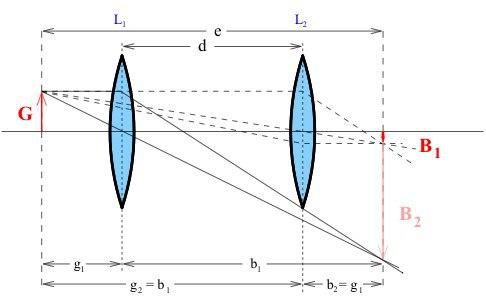
\includegraphics[width=0.6\textwidth]{bilder/bessel.jpg}
    \caption{Systematische Darstellung der Methodik\cite[4]{anleitung}}
\end{figure}
\label{sec:Durchfuehrung}
\subsection{Brennweitenbestimmung Abbe}
Hierbei wird die Brennweite und die Lage der Hauptebeneen aus dem Abbildungsmaßstab $V$ bestimmt.
Hierfür wird die Bildweite $b$ und die Gegenstandsweite $g$ relativ zur jeweiligen Hauptachse $H$ und $H'$ gemessen.
Da diese unbekannt sind wählt man einen beliebigen Punkt $A$.\\
Man misst nun die Bildweite $b'$ und die Gegenstandsweite $g'$, es gilt
\begin{align}
    g'=g+h=f \cdot \left(1+\frac{1}{V}\right)+h, \label{eqn:abbe1}\\
    b'=b+h'=f \cdot \left(1+V\right)+h'. \label{eqn:abbe2}
\end{align}
Die Linsen werden dabei auf der optischen Bahn direkt nebeneinander gestellt, sodass sie gemeinsam bewegt werden können,
ohne ihren Abstand zueinander zu verändert. Nun wird $V$, $b'$ und $g'$ gemessen.
